% This document is for a tutorial video
%https://www.overleaf.com/learn/latex/LaTeX_video_tutorial_for_beginners_(video_1)

% All \ are Laytek commands

\documentclass[letterpaper,12pt]{article}  % Tells what type of document you want to make. Article is useful for scientific journal.
% https://www.youtube.com/watch?v=CxOCIfQhFmI&ab_channel=ShareLaTeX
% If you want a longer option you can use book or Journal class
% Can add chapters, split up documents into multiple files
\usepackage{tabularx} % extra features for tabular environment

\usepackage[utf8]{inputenc}  % lets you use accented UTF8 characters
\usepackage{amsmath}  % amsmath for more math options
\usepackage{graphicx}  % graphics package
\graphicspath{{Images/}}  % adds image path for putting in folder
% Bibtek is included automatically
%\usepackage[round]{natbib} % helps customize references
\usepackage[margin=1.25in,letterpaper]{geometry} % decreases margins
\usepackage{cite} % takes care of citations
\usepackage[final]{hyperref} % adds hyper links inside the generated PDF file
\hypersetup{
	colorlinks=true,       % false: boxed links; true: colored links
	linkcolor=blue,        % color of internal links
	citecolor=blue,        % color of links to bibliography
	filecolor=magenta,     % color of file links
	urlcolor=blue
}
\usepackage{blindtext}
\usepackage{fancyhdr}
\usepackage{enumitem}
\usepackage{sectsty}

\sectionfont{\fontsize{12}{12}\selectfont}

% \usepackage{natbib}  % Used for fancier biliography/citations
% \bibliographystyle{plainnat}  % the style setup
%\setlist{itemsep=1pt,leftmargin=*}

% Inserts key turns on and off text insert mode


%++++++++++++++++++++++++++++++++++++++++
% Decided not to do traditional title because it took to much space
% Using fancy header formatting https://www.overleaf.com/learn/latex/headers_and_footers#Standard_page_styles

\pagestyle{fancy}
\fancyhf{}
\rhead{CSE 701 -  Final Project - NPC Racer \newline Brendan Fallon}
\lhead{December 9, 2022}  % April 14, 2021
\rfoot{Page \thepage}
\lfoot{}

\title{ % Make subtitle lines with \\
    NPC Racer \\
    \large A Computational Comparison of Game Pathfinding Algorithms. \\
    CAS 701 - Foundations of Modern Scientific Programming - \\
    Final Project}
\date{Friday, December 9, 2022} %Wednesday, April 14, 2021
\author{Brendan Fallon}

%++++++++++++++++++++++++++++++++++++++++

% This is all preamble

\begin{document}  % Always need begin and end

\maketitle  % This makes the title of the document from the preamble

\tableofcontents  % makes a table of contents

\section{Acronyms and Project Constraints}

\subsection{Project constraints}

\begin{itemize}
	\item The project must be implemented completely in C++ and GCC
	\item  The project has to contain only your code (no libraries)
	\item  The project must be somewhat related to your research or physics
	\item  Must follow the requirements on the 
	\href[]{https://baraksh.com/CSE701/#toc-guidelines}{course website} 
\end{itemize}




\subsection{Acronyms}

\begin{itemize}
	\item AI – Artificial Intelligence, concerning video games the branch of 
	computation 
	related to mimicking certain human behaviour in a game environment \cite{ 
		millingtonAIGamesThird2019}
	\item NPC – nonplayable character, concerning video games a character that 
	is not 
	directly controlled by the player and usually by the computer itself \cite{ 
		millingtonAIGamesThird2019}
\end{itemize}




\section{Purpose}
This final project should be a culmination of our understanding of not only C++ 
but good quality portable code taught in class. It should also be of sufficient 
complexity to be considered for a graduate-level final project. For this 
project, I’ve decided to do a performance comparison of video game pathfinding 
algorithms. This document will take you through a background of video game 
NPCs, the theory of pathfinding algorithms, an outline of the project, and the 
intended implementation. 

\section{Introduction}
Why is this important?

Non-playable characters (NPCs) or artificial intelligence (AI) in video games 
make up a significant portion of the game experience of many games. To simulate 
intelligent navigation, AI generally will move with respect to a specific 
target, say for example towards or away from the character. To do this they 
implement a form of pathfinding to calculate how to efficiently get to the 
target. Video games are an interesting application because there are timing 
requirements that state when the program should produce a result. For example, 
if a game is frame rate controlled, running at 144 Hz (144 frames per second) 
you only have 6.94 milliseconds to complete all the operations for each frame. 
For computers that do operations on the nanosecond timescale, this may seem 
like an eternity. But when you factor in that you need to do all the 
computationally expensive game logic, physics, graphics, sound, etc there is 
very little time left over for the AI to do calculations. This means that we 
need to be able to be as computationally efficient as possible when it comes to 
AI pathfinding. To do this we must pick an algorithm that is as efficient as 
possible. 

\section{Pathfinding Algorithms}
\label{section:Pathfinding_Algorithms}
How do these algorithms work?

Algorithms for pathfinding have been well-established since the dawn of 
computing. For example, the travelling salesman problem has many possible 
solutions \cite{ TravellingSalesmanProblem2022}. In computer science, we like 
to think of these algorithms as working on a weighted directed graph. Meaning 
that we have a series of nodes, edges that connect those nodes, weights on each 
of those edges, and a direction for each edge. For example, we could easily 
represent a road map as a series of intersections (nodes), roads (edges), road 
lengths (weights), and whether the street is one-way or two-way (direction). We 
would start at a certain node and have a destination ending up at another 
particular node on the graph. The goal is then to figure out which series of 
edges would be the shortest total weighting to get there.

% big O notion in Latex reference: 
%https://texblog.org/2014/06/24/big-o-and-related-notations-in-latex/
% Using Big Theta, $\Theta$ as in the Wikipedia reference
% Apparently Big Theta means the tightest bound! Good to know!
%https://www.geeksforgeeks.org/difference-between-big-oh-big-omega-and-big-theta/
% Using fancy big O where not big theta $\mathcal{O}(n\log{}n)$

One of the simplest, but very inefficient, ways to compute the shortest path is 
to brute force it. You could imagine computing every variation of every path 
possible from the source to the destination and picking the one with the 
shortest distance. The time complexity of this is horrible at a big O of 
$\mathcal{O}(n!)$ where n is the number of nodes in the graph 
\cite{TravellingSalesmanProblem2022}. A more efficient algorithm is Dijkstra’s 
algorithm. In short, Dijkstra looks through paths efficiently by dynamically 
deciding to stop looking through branches of paths when they have already been 
visited as well as continuing looking down the shortest branch seen so far 
first. The performance of this algorithm is already significantly faster than 
brute force. The complexity is dependent on the data structure used but with 
arrays you can reach $\Theta(|V|^2)$ and with a priority queue/heap you can 
reach a  $\Theta(|E| + |V|log|V|)$, where $|V|$ is the number of 
vertices/nodes and $|E|$ is the number of edges \cite{DijkstraAlgorithm2022}.

However, one flaw of Dijkstra’s algorithm is it doesn’t necessarily consider 
the if each path moves toward the destination. It could start going off on a 
series of edges that are short but in completely the wrong direction. In this 
way, Dijkstra’s algorithm has no heuristic for what a good path is. For highly 
non-uniform and sparse graphs, such as road networks, this is okay. However, if 
the graph is a grid, as in the case with video game spaces, then each edge has 
equal weighting and it must search in all directions because each direction is 
equally as short until it reaches the destination. To improve this an extension 
of Dijkstra’s algorithm was made known as the A* pathfinding algorithm. A* uses 
a heuristic, such as distance to destination, to make sure that each shortest 
path is in the best direction. For example, with A* you could use the 
Pythagorean theorem distance from each subsequent node to the destination to 
pick the next node to follow \cite{computerphileStarSearchAlgorithm2017}. When 
represented as a tree the performance of the A* pathfinding algorithm is 
$\mathcal{O}(|E|)$ or $\mathcal{O}(b^d)$ where b is the branching factor and d 
is the depth of the tree. However, the actual complexity is heavily dependent 
on the heuristic used \cite{SearchAlgorithm2022, AlgorithmsGraphSearch}.

It should be noted that there are \textbf{many} other pathfinding algorithms 
\cite{ShortestPathProblem2022 } work in various circumstances and purposes. 
Most of them however are not particularly relevant for gaming but could be 
applied nonetheless. The branch of heuristic algorithms is its own subfield 
including many nature-inspired algorithms like ant-colony optimization 
\cite{AntColonyOptimization2022} and bees algorithm \cite{ BeesAlgorithm2022}. 
For our comparison, we will be starting with the three algorithms above because 
they are the simplest and most popular in the context of video games. Future 
work can include looking into more types of video game AI algorithms 
\cite{millingtonAIGamesThird2019}. 



\section{NPC Racer}
What is it going to do?

NPC racer at its heart will be a project to compare the computational times of 
common pathfinding algorithms for video games. We will use a simplistic 
representation of a video game space with paths and barriers which we will call 
a maze. Then we will measure the time it takes for an agent to compute the 
shortest path from its starting location to the destination, called a trial. 
Each of these time trials will be performed multiple times for each of the 
pathfinding algorithms (brute force, Dijkstra, and A*). Then a statistical 
analysis, taking the mean and standard deviation, will be done for a series of 
trials which we will call a run. From there we can compare the runs for each of 
these different algorithms to see which is the fastest and by how much, which 
we will call a race. We can then have races on different-sized mazes and with 
differing amounts of barriers testing the algorithms in differing conditions. 
In this way, we are racing different agents to see which one is the fastest 
which is where the name NPC Racer comes from. A summary is given below and a 
diagram in figure \ref{fig:hierarchy} can be used to illustrate the idea 
further. 

\begin{figure}[h]  % h for here, p for separate page, b\t, or !
	\centering  % centers the figure in the page
	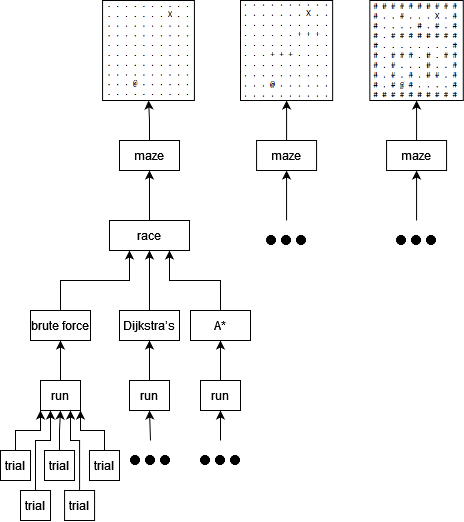
\includegraphics[width = 9 cm ]{NPC_Racer_Hierarchy.drawio.png}
	\caption{A diagram showing the hierarchy of tests and nomenclature for NPC 
	Racer.}
	\label{fig:hierarchy}
\end{figure}

\newpage

To summarize here:
\begin{itemize}
	\item A \textit{maze} is a space of paths, barriers, a starting point, and 
	a destination.
	\item For each \textit{maze}, a \textit{race} is done.
	\item For each \textit{race}, each of the algorithms is tested.
	\item For each algorithm, a \textit{run} is done.
	\item For each \textit{run}, a series of \textit{trials} are done
	\item Each \textit{trial} is a timed event where the agent solves a 
	\textit{maze} for the shortest path between the start and the destination.

\end{itemize}

The key to this project will be code consistency. The goal is not to make the 
fastest pathfinding algorithm possible but to compare them. As such we will 
have to be using consistent data structures and implementation methods for each 
algorithm to make sure the results are valid.


\section{Implementation}
How is it going to work?\footnote{Any of these implementation details could be 
	subject to change if when I make the program these don’t make sense or 
	don’t 
	work.}

Because this will be a significantly large program, we will be breaking up our 
project into four distinct modules each in its own separate file:

1.	Maze Class – Handling maze data storage/manipulation as well as maze IO 
with files.

2.	Agent Class – Pathfinding agent classes for finding the shortest path on a 
maze

3.	Timekeeper Classes – Chrono timing and trial/run/race statistics.

4.	Main – Setup and call all the classes to implement races on mazes with 
statistics then output the results to the terminal.

A visualization of how the modules interact can be seen in figure 
\ref{fig:modules}. Here you can see how all the modules interact including the 
separation of the namespace between the main class and the rest of the classes. 
This is so that in the main program we can easily distinguish what is from the 
NPC Racer project and what is from the standard library. It also allows 
bundling these modules together for any future projects that don’t involve maze 
racing. Each module should also be very abstract from the rest of the modules. 
I.e. if the maze class was changed then it should not change the implementation 
in the main program or agent class. They should be able to work effectively 
through each other’s interfaces. Each module will be expanded upon below. 

\begin{figure}[h]  % h for here, p for separate page, b\t, or !
	\centering  % centers the figure in the page
	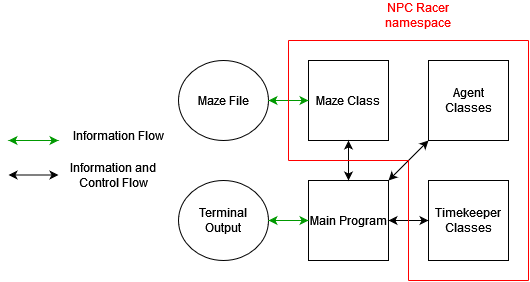
\includegraphics[width = 9 cm ]{NPC_Racer_System_Modules.drawio.png}
	\caption{The NPC Racer system module interaction diagram.}
	\label{fig:modules}
\end{figure}

\subsection{Maze Class}

Mazes offer a great testing point, especially for games, because they are 
densely populated, have many branching paths, and are easy to generate. Our 
maze structure will be made up of ASCII/UTF-8 characters with `.` denoting a 
free space, `@` denoting the starting location of the agent, and `X` or `x` 
denoting the destination of the agent. Any other single symbol, besides a comma 
or whitespace, will be treated as a wall or barrier. Therefore a valid path 
would travel along `.` from the `@` symbol to the `X` symbol. For consistency, 
each space or barrier must only be one character to make fixed-width printing 
easier. These symbols were inspired by the original Rogue game from 1980 \cite{ 
RogueVideoGame2022}. The mazes in figure \ref{fig:mazes} a-c would all be valid.

\begin{figure}[h]  % h for here, p for separate page, b\t, or !
	\centering  % centers the figure in the page
	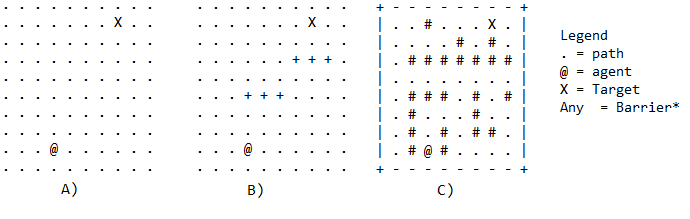
\includegraphics[width = 9 cm ]{NPC_Racer_Maze_Examples.png}
	\caption{Examples of 10x10 mazes a) An empty maze b) A maze with two 
	barriers c) a fully closed maze.}
	\label{fig:mazes}
\end{figure}

We could make it so mazes generate on the fly but that is out of the scope of 
this work. So for now we'll make the maps by hand or rely on other tools to 
generate mazes saved to a file. This means that the maze class will have to be 
able to read mazes from a file as its constructor. It would also be ideal if it 
could write a default empty maze to files to create future mazes.

\subsection{Agent Classes}
We will define a generic prototype agent class that implements the basics of 
reading spaces of mazes. From there we can derive classes for each algorithm 
which will make the concrete implementation of the pathfind method. Then we can 
use polymorphism to call the same method no matter what algorithm is being 
used. For each of the algorithms, the underlying datatype we will be using are 
vector containers from the STL library. These are not the fastest but should at 
least be easy and consistent if used between all the algorithms. The 
implementation of the brute force, Dijkstra’s, and A* algorithms will be 
similar to the high-level description in the 
\hyperref[section:Pathfinding_Algorithms]{Pathfinding algorithms} section. Any 
further differentiating details will be discussed in the coding documentation.


\subsection{Timekeeper Classes}
There will be 3 classes one for trials, one for runs, and one for races. Will 
be using the Chrono timer to time trials and the time will be kept in a vector 
for each run. From there we can use the algorithms library to get the mean and 
standard deviation of the run. We will also include a race as a map datatype so 
we can compare algorithm runs for each race. In theory, this does not need to 
be three distinct classes but could be a collection of useful functions. I’m 
not fully decided on this and it may be better to define it as a single static 
class that collects utility functions or just move all the methods to the main 
program.

\subsection{Main Program}
The main program will be responsible for setting up and calling all the classes 
to perform the races. Most likely it will take an argument from the command 
line for which maze to perform the race on. From there it will set up the 
algorithm agents and do a run for each. The timekeeper classes will keep track 
of the timing of everything and print out the statistics for each run and the 
race in total. Visualization of the agent pathfinding will be left for future 
work. For now, the program will output results to the terminal.
  


\addcontentsline{toc}{section}{References}  % adds a line to the table of contents, not done automatically
\bibliographystyle{plain}  % the style setup
%Enter the .bib style, can be plain or Plainnat with the nat package, can enter multiple filenames with coma
\bibliography{../NPC_Racer_Citations.bib}  
%https://tex.stackexchange.com/questions/29172/link-to-file-in-the-parent-folder

\newpage
\appendix  % adding an appendix

%\section{Appendix: The files}
%\label{appendix:files}  % section for reference
%This is the Appendix

%\section{Appendix: Project evolution}
%\label{appendix:files}  % section for reference
%The project evolved over various stages and ideas based on limiting scope/complexity, time constraints, technology limitations, etc. I included a few screenshots on %how the modelling process evolved.

%\section{Appendix: GMF EVL Integration Tutorial}
%\label{appendix:tutorial}  % section for reference


%\section{Appendix: Extending Generated Python Code Example}
%\label{appendix:pythoncode}  % section for reference







\end{document}

